\newpage
\section{Progettazione}
\subsection{Studio dell'utenza finale}
\subsubsection{Utente generico}
L'utenza maggiore che ci si aspetta potrà visitare questo sito è composta principalmente da persone dal profilo informatico medio basso alla ricerca di informazioni dettagliate riguardo la fornitura dell'azienda, probabilmente in mobilità. L'applicativo web offre informazioni relative ad un'azienda agricola, posto che in genere non è frequentato pubblicamente per svago. Per questo motivo la maggior parte delle informazioni sono contenute in pagine statiche. Inoltre si sono create le pagine di \textbf{servizi} e \textbf{prodotti} che, pur non permettendo un acquisto o una prenotazione on line, offrono all'utente la possibilità di vedere le offerte e di contattare l'azienda telefonicamente nella scheda \textbf{contattaci}.
\subsubsection{Azienda business-to-business}
Ci si può aspettare inoltre che qualche azienda in cerca di un commercio business-to-business di grano visiti il sito. In questo caso le pagine statiche di \textbf{home} e \textbf{chi siamo} offrono una panoramica sulla storia e sulla solidità dell'azienda, pubblicizzandola. Ci si aspetta quindi un utente più esperto nell'utilizzo di un PC o smartphone, che quindi potrà eventualmente anche creare un messaggio con più informazioni, in attesa di un contatto telematico, sfruttando il form preparato nella scheda \textbf{contattaci}.
\subsubsection{Amministratore}
Il sito potrà essere gestito da uno o più amministratori ingaggiati dall'azienda, che si supporranno essere persone mediamente più esperte nell'utilizzo di un computer, che si occuperanno di amministrare il sito da una postazione principalmente fissa.

\subsection{Layout del sito}
Sebbene abbastanza simili sotto il punto di vista del layout, la struttura presentata agli utenti generici e agli amministratori varia di un po'. Prenderemo in esame i due layout in maniera distinta.
\subsubsection{Utente generico}
\paragraph{Barra di navigazione}
~\\Il sito è stato pensato per avere una navigazione a barra orizzontale fissa posta in alto sullo schermo. Le pagine del sito sono, per quanto riguarda gli utenti non registrati:
\begin{itemize}
	\item \textbf{Home}
	\item \textbf{Chi siamo}
	\item \textbf{Prodotti}
	\item \textbf{Servizi}
	\item \textbf{Contattaci}
\end{itemize}
Nella barra è presente il logo dell'azienda e i pulsanti che portano alle altre pagine del sito. In particolare, il pulsante indicante la pagina attuale è incorniciato, mentre gli altri, se il mouse ci passa sopra, vengono sottolineati. All'interno della barra, posto subito sotto, è presente il breadcrumb: a sinistra si occupa di indicare la posizione attuale all'interno del sito, a destra è presente un'ancora che porta direttamente al contenuto. Se si utilizza il \emph{tab} da tastiera si potrà apprezzare che questo è il primo link cliccabile. Nell'immagine seguente è possibile vedere un esempio della barra:
\begin{figure}[h!]
	\centerline{
\includegraphics[scale=0.45]{img/barra_navigazione.jpg}}
	\caption{Barra di navigazione per l'utente generico}
	\label{fig:navbarGU}
\end{figure}
~\\Sebbene non facente parte della barra, è presente un'àncora fissata in basso a destra sul sito che si occupa di riportare il lettore all'inizio del contenuto.
\begin{figure}[h!]
	\centerline{
\includegraphics[scale=0.45]{img/jump_to_menu.jpg}}
	\caption{Ancora all'inizio del contenuto}
	\label{fig:anchor}
\end{figure}
\paragraph{Corpo}
~\\Il corpo è disposto con layout orizzontale all'interno della pagina, con una larghezza massima fissata, in modo da renderlo più elegante anche con risoluzioni elevate. La maggior parte dei contenuti è organizzata in rettangoli, ognuno dei quali contiene il titolo della sotto sezione, il testo e un'immagine indicativa.
Nell'immagine subito successiva si può notare un esempio:
\begin{figure}[h!]
	\centerline{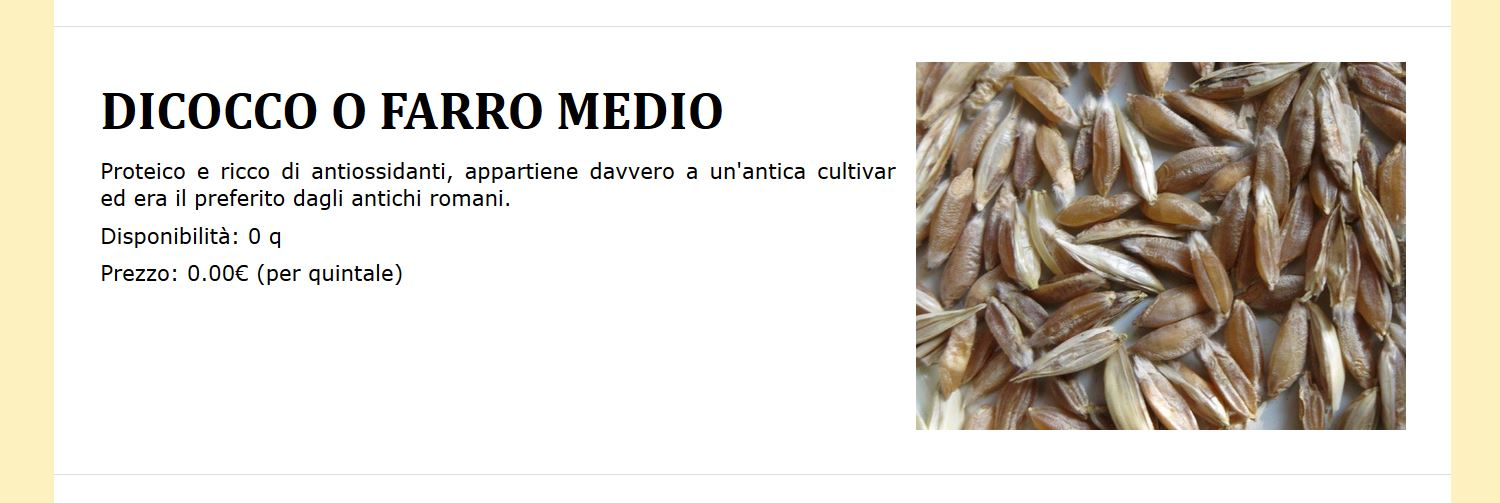
\includegraphics[scale=0.40]{img/corpo_esempio.jpg}}
	\caption{Esempio di sezione del corpo}
	\label{fig:corpoGU}
\end{figure}
\paragraph{Pié di pagina}
~\\A pié di pagina si possono trovare delle informazioni relative al progetto, ovvero il nome dei partecipanti alla creazione del sito e le certificazioni di adesione agli standard \emph{XHTML} e \emph{CSS3}. Inoltre è presente un collegamento alla sezione di amministrazione, alla quale si può accede solo se già registrati da un altro amministratore.
\begin{figure}[h!]
	\centerline{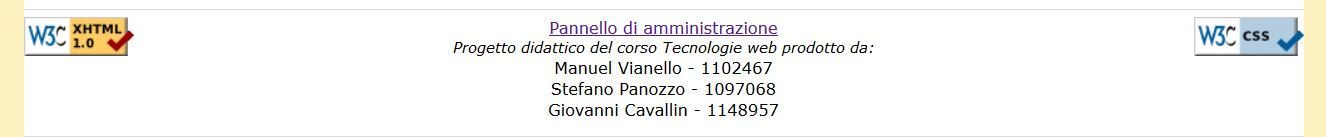
\includegraphics[scale=0.45]{img/footer.jpg}}
	\caption{Pié di pagina del sito}
	\label{fig:footer}
\end{figure}
\subsubsection{Amministratore}
La GUI si differenzia da quella dell'utente base per alcune particolarità.
\paragraph{Barra di navigazione}
~\\Al posto delle pagine sopra illustrate ci sono altre pagine in cui navigare:
\begin{itemize}
	\item \textbf{Pannello amministrazione}
	\item \textbf{Prodotti}
	\item \textbf{Servizi}
	\item \textbf{Storico prenotazioni}
	\item \textbf{Prenotazioni}
	\item \textbf{Clienti}
	\item \textbf{Amministratori}
\end{itemize}
Nel breadcrumb poi, al posto del \emph{Vai al contenuto}, sono presenti due link: un \emph{Torna al sito} e un pulsante di \emph{Logout}, che hanno lo stesso risultato di riportare l'utente al sito generico, ma che nel secondo caso chiude la sessione di amministratore. Viene infine rimossa l'àncora per tornare all'inizio della pagina.
\begin{figure}[h!]
	\centerline{
\includegraphics[scale=0.49]{img/barra_navigazione_admin.jpg}}
	\caption{Barra di navigazione per l'amministratore}
	\label{fig:navbarAD}
\end{figure}
\paragraph{Corpo}
~\\La struttura rimane pressoché invariata, ma in ognuna di esse - meno la \textbf{Storico prenotazioni} - è presente a fondo pagina un modulo di aggiunta informazioni.
\begin{figure}[h!]
	\centerline{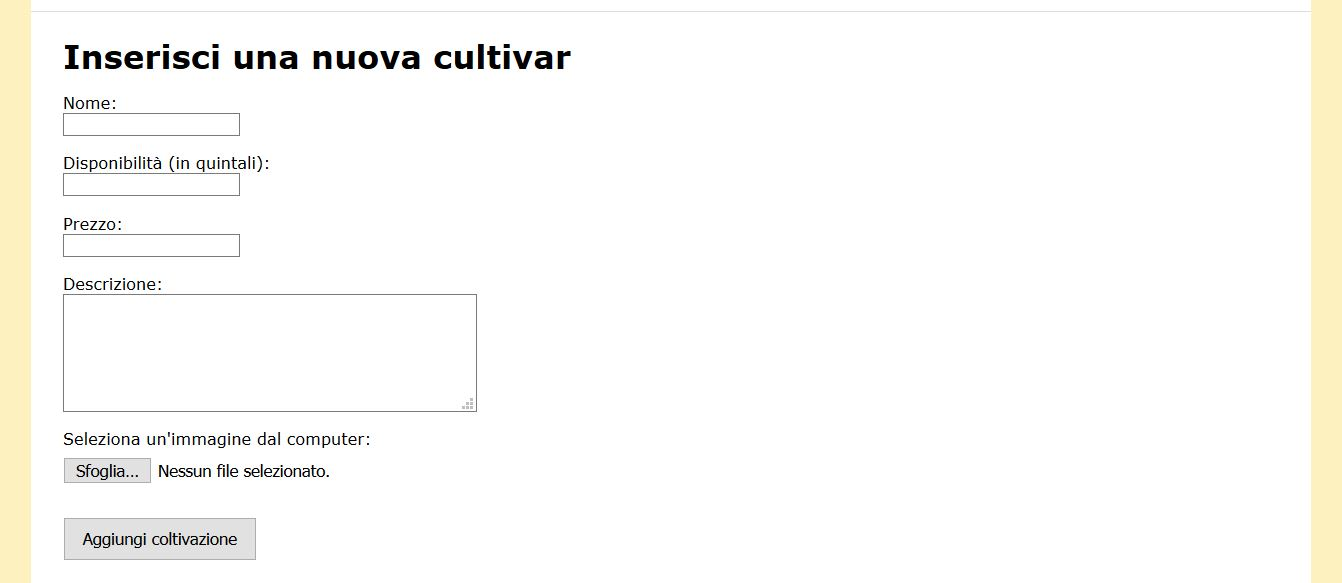
\includegraphics[scale=0.49]{img/add_form.jpg}}
	\caption{Form di aggiunta informazioni}
	\label{fig:addForm}
\end{figure}
\paragraph{Pié di pagina}
~\\Nel pié di pagina invece viene solamente rimosso il link al pannello di amministrazione poiché inutile.

\subsection{Contenuti veicolati}
Dal punto di vista dei contenuti veicolati invece il sito presenta una profonda differenza a seconda del destinatario a cui si riferisce. Prenderemo in esame un utente alla volta.
\subsubsection{Utente generico}
I contenuti destinati all'utente generico possono essere statici o dinamici:
\paragraph{Contenuti statici}
\subparagraph{Home}
~\\È una rapida overview delle informazioni relative all'azienda. Quindi è presente il logo, che la identifica anche visivamente, e un riepilogo di come l'azienda si preoccupa di coltivare i propri prodotti.
\subparagraph{Chi siamo}
~\\È una presentazione un po' più approfondita dell'azienda, dove vengono descritte le origini della stessa e la sua mission, per così dire, ovvero l'agricoltura biologica.
\subparagraph{Contattaci}
~\\È una pagina dei contatti, dove l'utente può mettersi direttamente in contatto con l'azienda attraverso un form da compilare, oppure potendo chiamare il numero di telefono disponibile. Per utilizzare il form è necessario che nel server in cui è hostato il sito sia predisposto un mail server. Come conferma dell'effettivo invio del form, si riceverà una copia della richiesta appena effettuata all'azienda Cavallin. Eventualmente è comunque possibile utilizzare il link sottostante oppure il numero di telefono.
\paragraph{Contenuti dinamici}
\subparagraph{Prodotti} 
~\\Presenta tutti i prodotti di cui l'azienda dispone al momento attuale e dei quali si occupa della coltivazione. Essendo possibile per l'azienda variare coltivazioni, si è pensato di rendere questi contenuti dinamici così da poterli aggiuntere, rimuovere o aggiornare dall'amministrazione. Sono correlati dal nome, una breve descrizione, un'immagine significativa, il prezzo al quintale e dalla disponibilità.
\subparagraph{Servizi} 
~\\Offre una visione delle attrezzature delle quali l'azienda dispone. Essendo disponibile un servizio da terzista, un eventuale cliente può vedere gli attrezzi e poi accordarsi con l'azienda attraverso il form di contatti. Questa parte verrà descritta nella parte di amministrazione.

\subsubsection{Amministrazione}
I contenuti destinati all'amministrazione sono solamente dinamici, poiché fortemente legati allo stato dei prodotti, dei servizi e delle prenotazioni. Un amministrazione ha a disposizione le pagine di:
\paragraph{Pannello amministrazione} viene presentata un riassunto di ciò che è possibile fare accedendo alla parte amministrativa del sito.
\paragraph{Prodotti}
~\\Viene visualizzata la lista dei prodotti attualmente disponibili ma senza immagini, poiché non troppo rilevanti al fine delle modifiche. Per ogni prodotto è possibile impostarne un nuovo prezzo al quintale e una nuova disponibilità. Inoltre è possibile eliminare la cultivar, qualora non ce ne fosse più bisogno, e aggiungerne una nuova, per la quale è necessario inserire tutti i campi disponibili: Nome, quantità, prezzo e un'immagine.
\paragraph{Servizi}
~\\Viene visualizzata la lista dei macchinari attualmente presenti in azienda. Come per i prodotti, è possibile modificarne il prezzo all'ora, si possono eliminare e se ne possono inserire di nuovi, compilando tutti i campi del form a fondo pagina.
\paragraph{Amministratori}
~\\È possibile per gli amministratori la gestione degli altri amministratori, che possono quindi essere aggiunti o eliminati in questa pagina.
\paragraph{Clienti}
~\\La parte amministrativa del sito permette la gestione di ordini di macchinari da parte di clienti per una certa quantità di tempo. Per questo motivo è presente una sezione \textbf{Clienti}, che si occupa di aggiungere tutte le informazioni relative ad un cliente che precedentemente si è dimostrato interessato all'azienda, e attraverso il quale poi è possibile effettuare la prenotazione vera e propria, che quindi attesta l'utilizzo di un determinato servizio da parte di un cliente ben preciso.
\paragraph{Prenotazioni}
~\\Qui si possono visualizzare le prenotazioni attualmente attive, oppure se ne può aggiungere una nuova: in questo caso bisogna selezionare il macchinario, sincerarsi della sua disponibilità, selezionare un cliente e le date di inizio e fine della richiesta. Non si possono ovviamente selezionare servizi attualmente attivi.
\paragraph{Storico prenotazioni}
~\\In questa sezione si possono visualizzare le prenotazioni passate: in questa maniera si può avere uno storico, utile per il gestore dell'azienda. Ovviamente quese prenotazioni non influiscono sullo stato dei macchinari, che quindi possono essere selezionabili durante la generazione di una prenotazione.











